% Asset ID: AS1VectorsTikZ-007
% Source: P1-Chp11-Vectors.pdf, Direction of vectors and bearings examples
% Related lesson section: Core Theory: Direction; Worked Example 16; Exam Technique
% Purpose: Show how a bearing is resolved into east and north components.
\documentclass[tikz,border=8pt]{standalone}
\usepackage{amsmath}
\usepackage{bm}
\usetikzlibrary{arrows.meta,positioning,angles,quotes}
\begin{document}

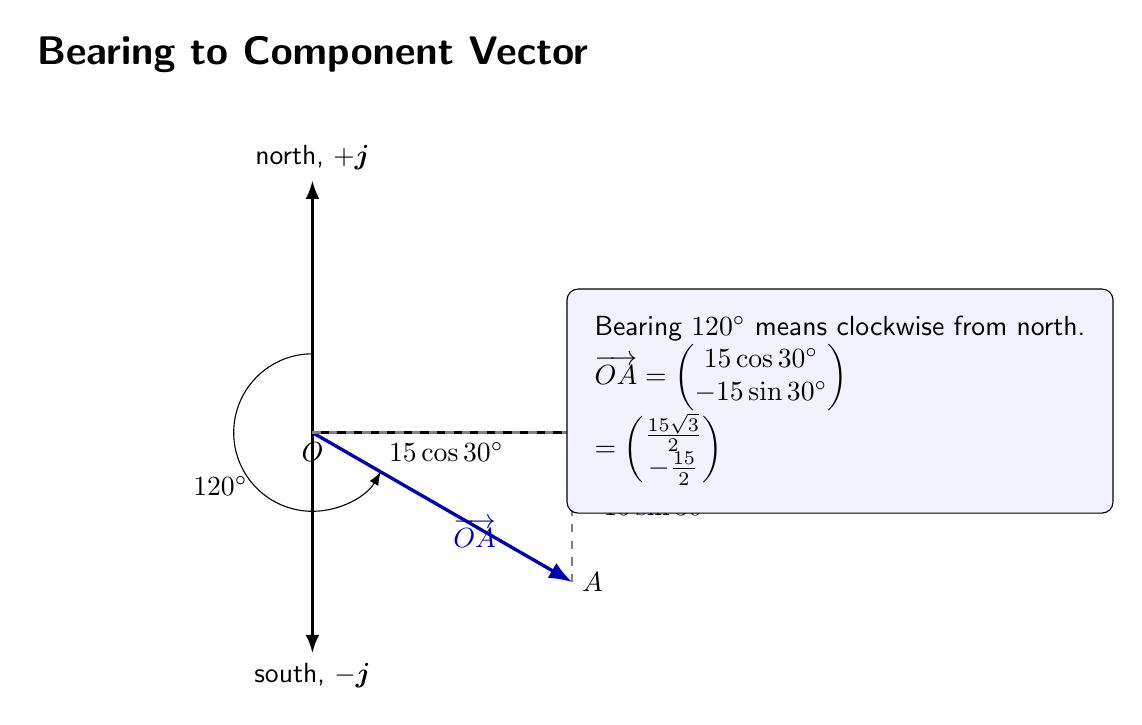
\begin{tikzpicture}[>=Latex,every node/.style={font=\sffamily},axis/.style={->,thick},vector/.style={->,very thick,blue!70!black},comp/.style={thick,dashed,gray}]
\node[font=\sffamily\bfseries\Large] at (0,4.8) {Bearing to Component Vector};
\coordinate (O) at (0,0);\coordinate (N) at (0,3.2);\coordinate (E) at (4,0);\coordinate (A) at (3.3,-1.9);
\draw[axis] (O)--(N) node[above] {north, $+\bm j$};\draw[axis] (O)--(E) node[right] {east, $+\bm i$};\draw[axis] (O)--(0,-2.8) node[below] {south, $-\bm j$};
\draw[vector] (O)--node[below right] {$\overrightarrow{OA}$}(A);\node[below] at (O) {$O$};\node[right] at (A) {$A$};
\draw[comp] (A)--(3.3,0);\draw[comp] (O)--(3.3,0);\node[below] at (1.7,0) {$15\cos30^\circ$};\node[right] at (3.3,-.95) {$-15\sin30^\circ$};
\draw pic[draw,->,angle radius=1cm,angle eccentricity=1.35,"$120^\circ$"] {angle=N--O--A};
\node[draw,rounded corners,fill=blue!5,align=left,inner sep=10pt] at (6.7,.4) {Bearing $120^\circ$ means clockwise from north.\\$\overrightarrow{OA}=\begin{pmatrix}15\cos30^\circ\\-15\sin30^\circ\end{pmatrix}$\\$=\begin{pmatrix}\frac{15\sqrt3}{2}\\-\frac{15}{2}\end{pmatrix}$};
\end{tikzpicture}

\end{document}
